\section{Fraktální dimenze}\label{sec:fraktalni_dimenze}
Výčet útvarů v sekci \ref{sec:sobepodobnost} splňoval zásadní vlastnost, a to sice, že všechny z nich byly \emph{soběpodobné}. V eukleidovské geometrii lze však u mnohých základních objektů pozorovat stejnou vlastnost. Např. čtverec lze určitě prohlásit v jistém smyslu za soběpodobný, neboť jej lze rozdělit na podobné útvary (viz obrázek \ref{fig:sobepodobnost-ctverce}).
\begin{figure}[h]
    \centering
    \begin{subfigure}[b]{\subfigwidth}
        \centering
        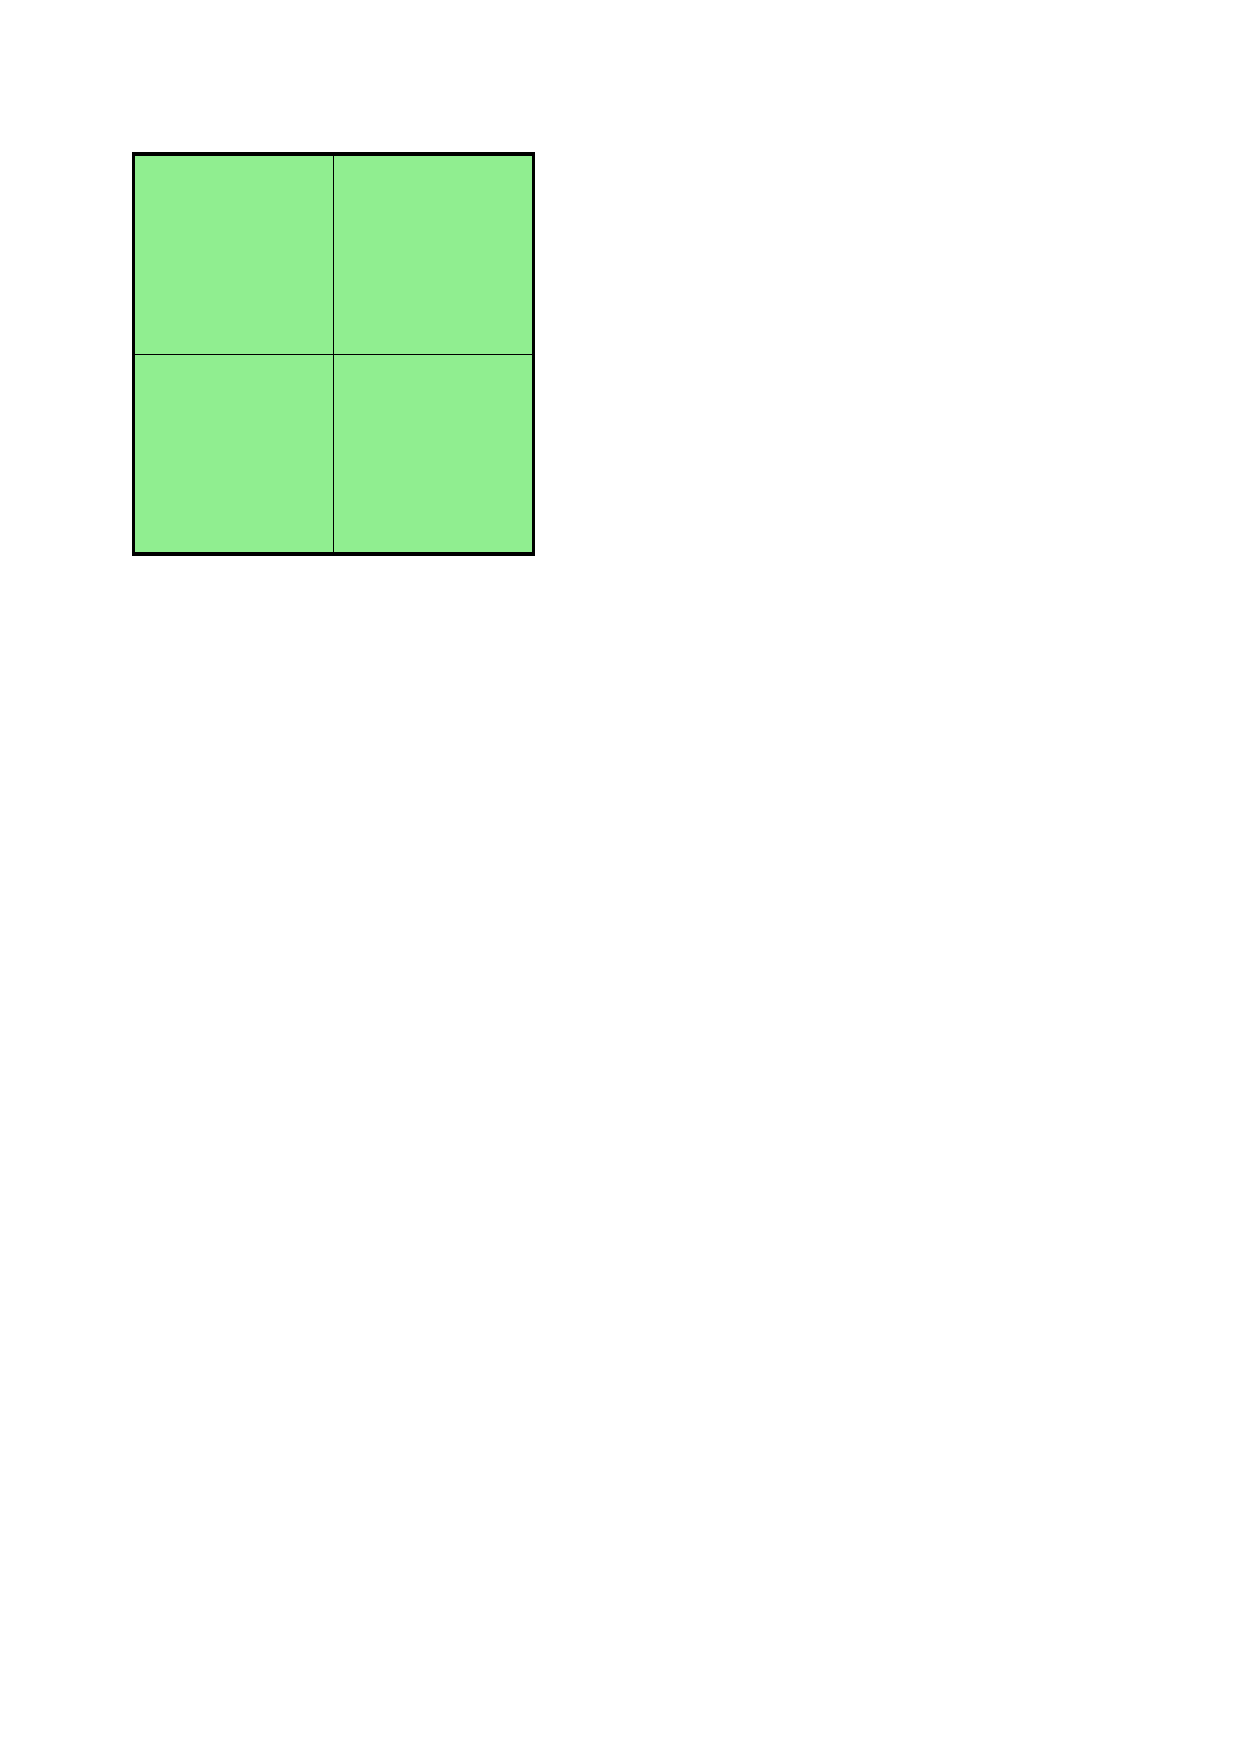
\includegraphics[scale=\normalipe]{ch01_ctverec_sobepodobnost.pdf}
        \caption{Čtverec rozdělený na čtyři menší čtverce.}
        \label{subfig:sobepodobnost-ctverce-1}
    \end{subfigure}
    \begin{subfigure}[b]{\subfigwidth}
        \centering
        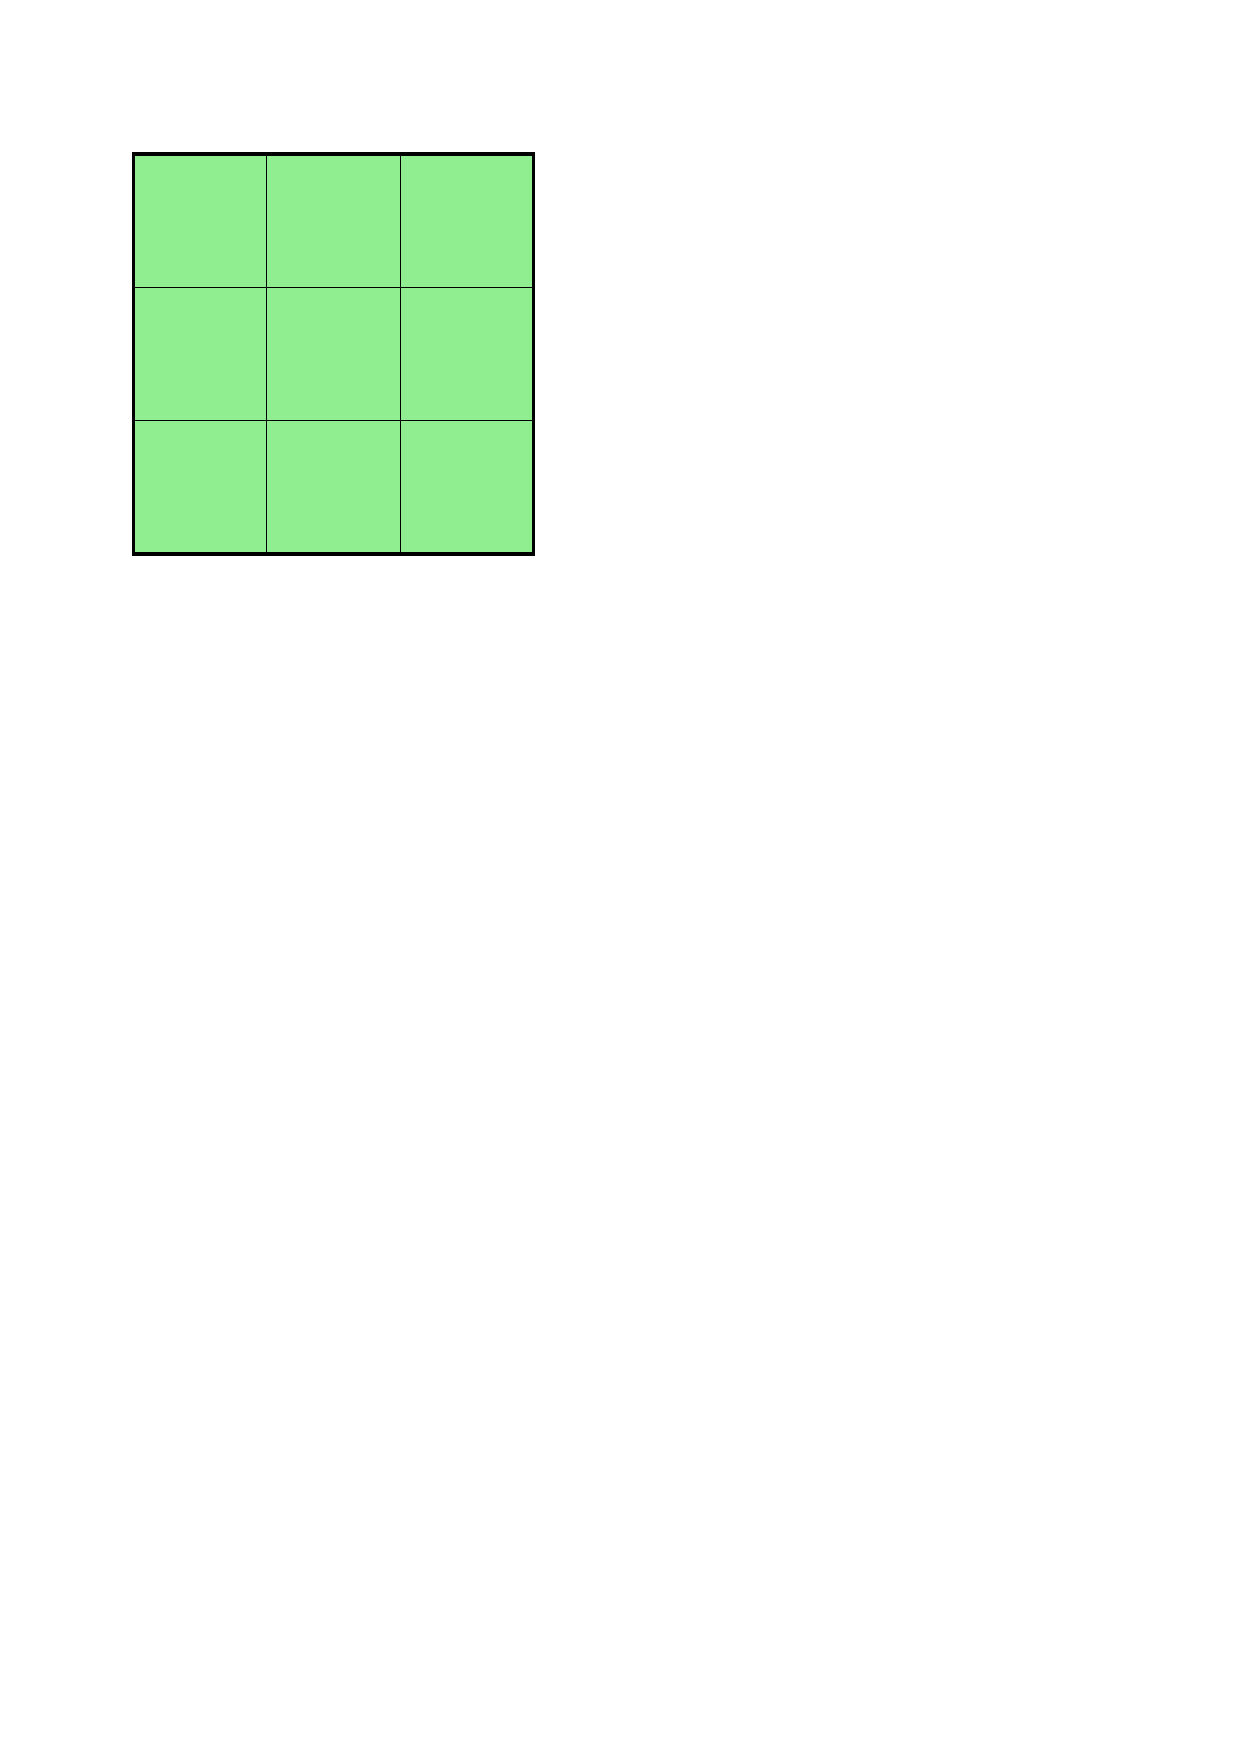
\includegraphics[scale=\normalipe]{ch01_ctverec_sobepodobnost_2.pdf}
        \caption{Jiná možnost rozdělení čtverce.}
        \label{subfig:sobepodobnost-ctverce-2}
    \end{subfigure}
    \caption{Soběpodobnost čtverce.}
    \label{fig:sobepodobnost-ctverce}
\end{figure}
Podobně např. i obyčejná úsečka je taktéž soběpodobná, protože ji můžeme rozdělit na obecně $k$ stejných částí (viz obrázek).\par
\begin{figure}[h]
    \centering
    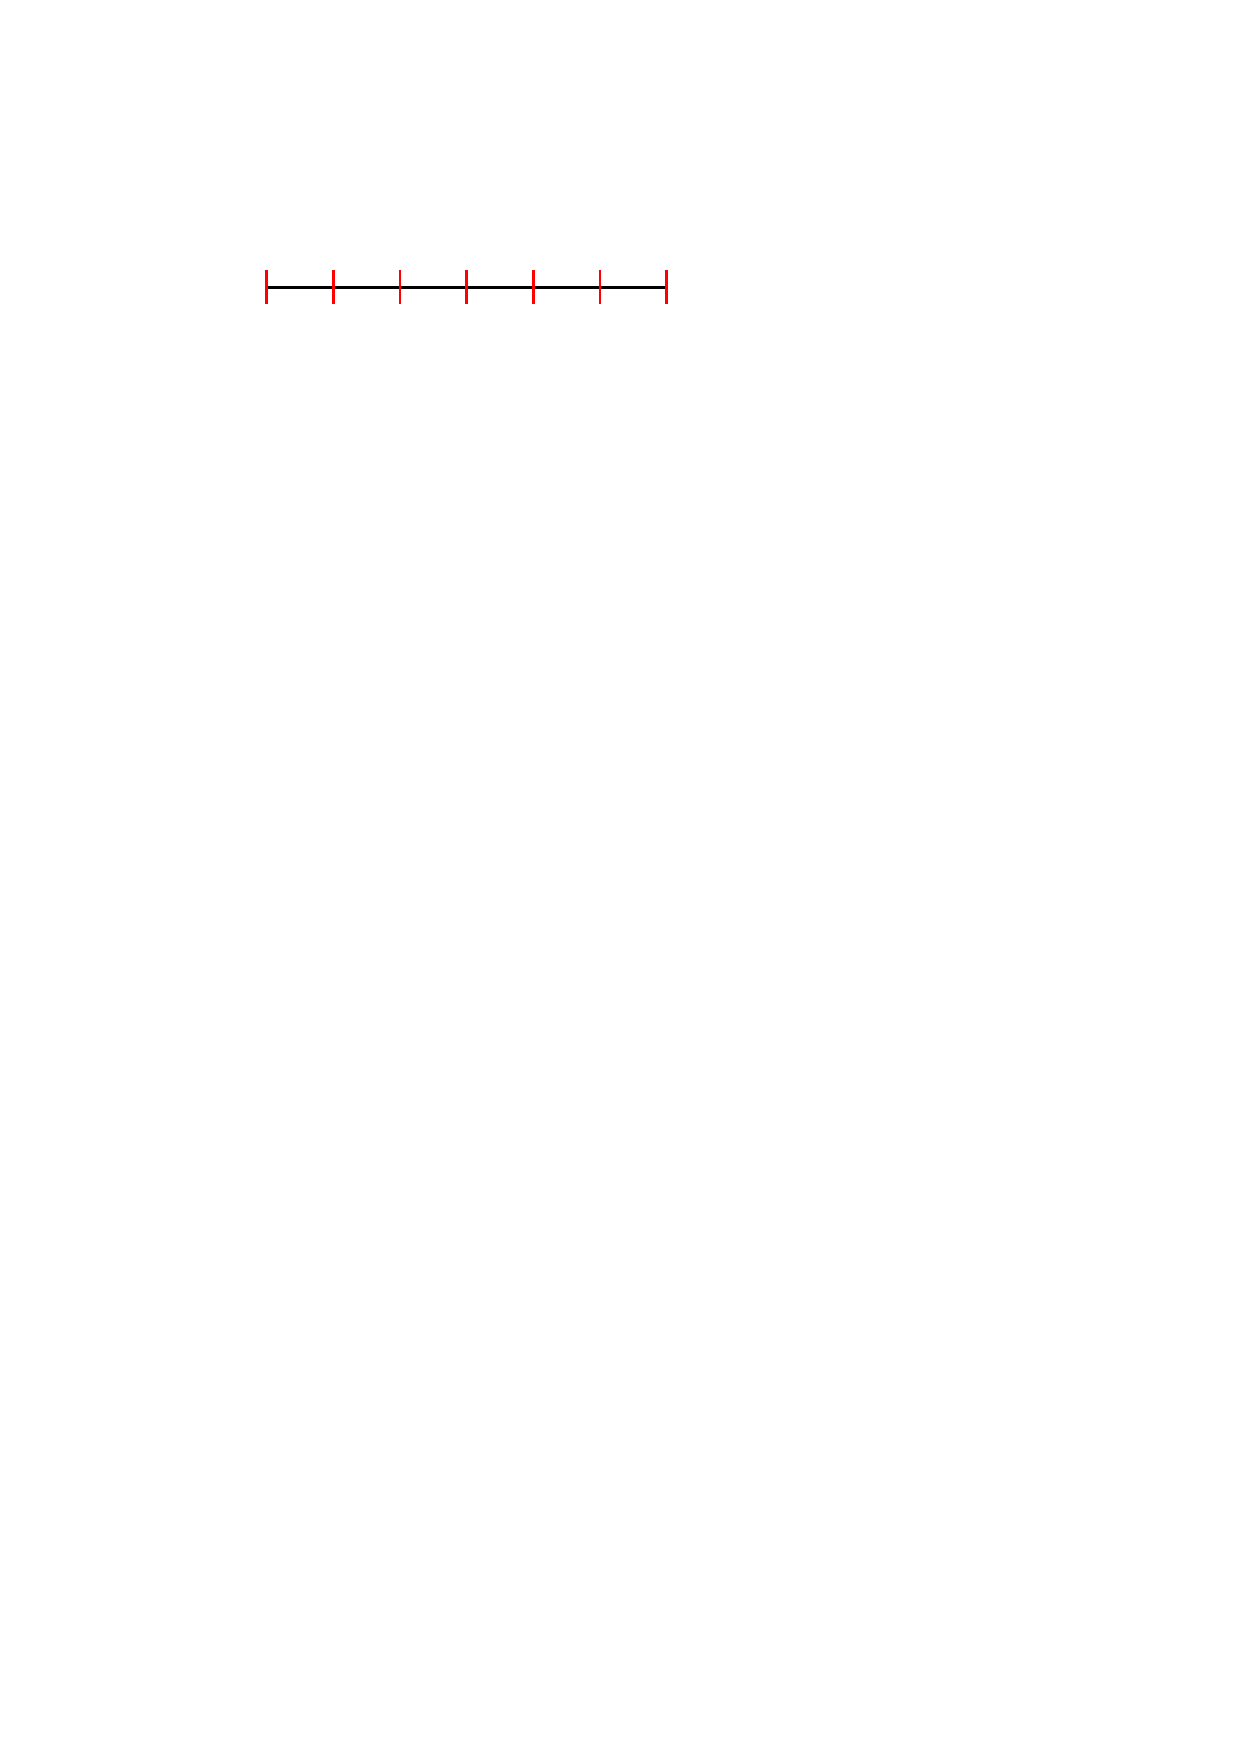
\includegraphics[scale=\normalipe]{ch01_usecka_sobepodobnost.pdf}
    \caption{Úsečka rozdělená na šest stejných částí.}
\end{figure}
K čemu nám takové uvědomnění vlastně je? Zmenšíme-li úsečku $k$-krát, pak budeme potřebovat přesně $k$ těchto částí, abychom dostali úsečku původní délky. U čtverce (nebo obdélkuníku obecně) při změnšení délky strany $k$-krát budeme potřebovat $k^2$ daných útvarů pro obdržení čtverce s původním obsahem.\footnote{Obdélník změnšený $k$-krát bude mít strany délek $a/k,\,b/k$, tedy jeho obsah bude
\[\dfrac{ab}{k^2}=\dfrac{S}{k^2},\]
kde $S$ je obsah původního obdélníka.}
Pro krychli bude situace zcela analogická, $k$-krát zmenšená kopie bude potřeba $k^3$-krát, abychom dostali krychli o původním objemu (viz obrázek \ref{fig:krychle-sobepodobnost}).
\begin{figure}[h]
    \centering
    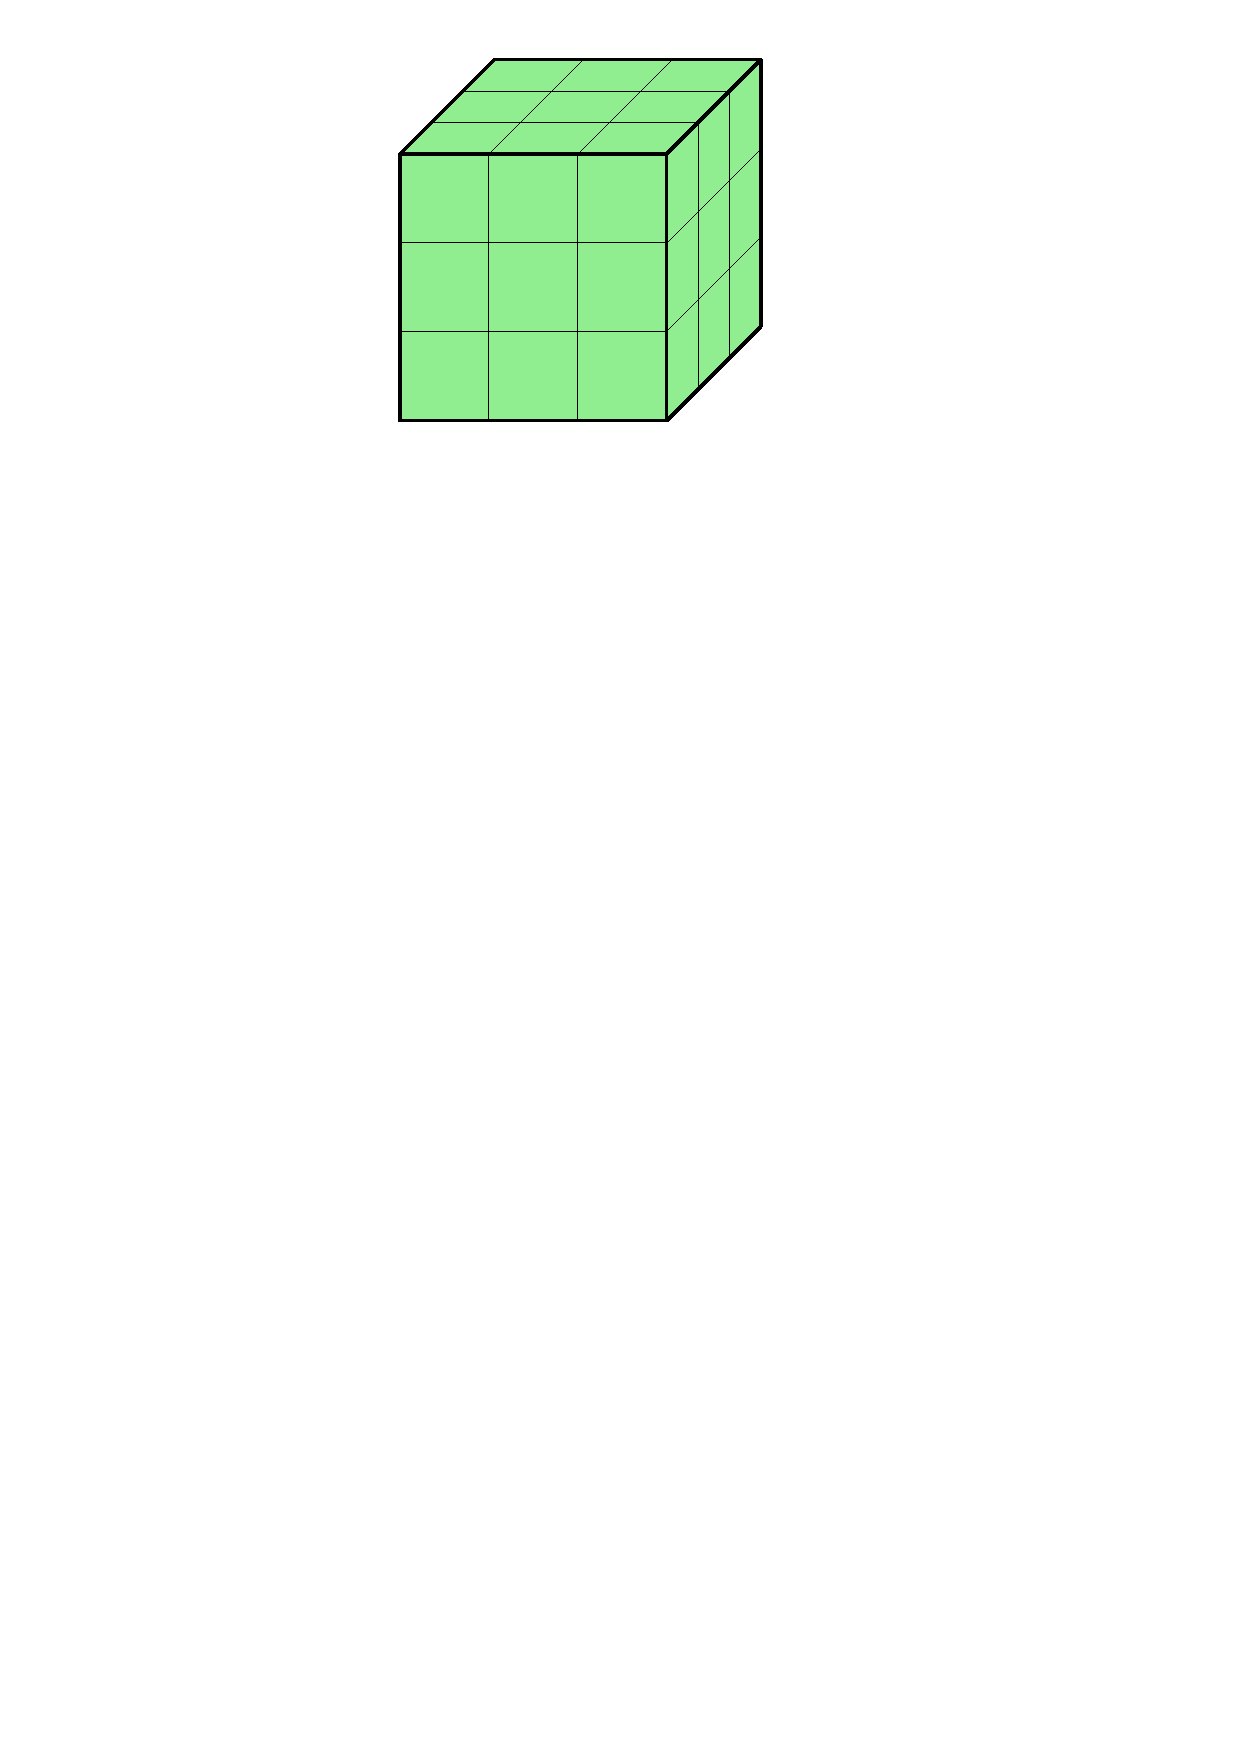
\includegraphics[scale=\normalipe]{ch01_krychle_sobepodobnost.pdf}
    \caption{Krychle rozdělená na 27 stejných částí.}
    \label{fig:krychle-sobepodobnost}
\end{figure}
Lze si všimnout, že v závislosti na \emph{dimenzi} objektu se mění daný exponent. Vztah lze tak zobecnit na
\begin{equation}\label{eq:pocet-utvaru}
    N(k)=k^d
\end{equation}
kde $N(k)$ je počet nových útvarů v závislosti na faktoru $k$ a $d$ je dimenze.\par
Čtenář si již nyní může všimnout, že toto je jeden z možných způsobů, jak lze chápat koncept dimenze.\footnote{Znalec lineární algebry by se nyní mohl pozastavit, neboť dimenze se zde definuje jako \emph{mohutnost libovolné báze vektorového prostoru} (v tomto případě $\R^n$, pro $n\in\N$), avšak lze si rozmyslet, že se z geometrického hlediska jedná o totéž.} Jednoduchou úpravou rovnosti \eqref{eq:pocet-utvaru} dostaneme
\[d=\log_k{N(k)}=\dfrac{\ln{N(k)}}{\ln{k}}.\]
(Obecně lze volit jakýkoliv přípustný základ logaritmů, tj $d=\log_b{N(k)}/\log_b{k}$ pro $b\in\R^+\setminus\set{1}$.)
\begin{table}[h]
    \centering
    \begin{tabular}{|l|c|c|}
    \hline
    Útvar    & $N(k)$ & $d=\log_3{N(k)}/\log_3{k}$ \\ \hline
    Úsečka   & $3$      & $1$                          \\ \hline
    Čtverec  & $9$      & $2$                          \\ \hline
    Krychle  & $27$     & $3$                          \\ \hline
    Teserakt\footnote{Čtyřrozměrná krychle} & $81$     & $4$                          \\ \hline
    \end{tabular}
    \label{table:eukleides-dimenze}
\end{table}
Dimenze v tomto pojetí skutečně dává dobrý smysl. Pro ``klasické'' geometrické objekty vychází dimenze vždy celočíselně.\par
Na této myšlence je založen pojem tzv. \emph{fraktální dimenze}\footnote{Někdy se též nazývá \emph{Kolmogorovova dimenze} nebo \emph{Hausdoffova-Besičovičova dimenze}. Je pojmenována po německém matematikovi \name{Felixi Hausdorffovi} (1869--1942) a ruských matematicích \name{Andreji Kolmogorovovi} (1903--1987) a \name{Abramovi Besičovičovi} (1891--1970).}, která je pro útvar definována jako
\begin{equation}\label{eq:fraktalni-dimenze}
    d_k=\lim_{\varepsilon\to 0^+}{\dfrac{\ln{N(\varepsilon)}}{\ln{\left(\dfrac{1}{\varepsilon}\right)}}}.
\end{equation}
(Převzato z \cite[str. 93]{Zelinka2006}.) Výraz $1/\varepsilon$ zde představuje faktor podobnosti jako původní $k$ (samotné $\varepsilon$ tak hraje roli měřítka), avšak největší rozdíl zde představuje zkoumání ``limitního chování'' daného výrazu.
\begin{example}[Fraktální dimenze úsečky]\label{ex:fraktalni-dimenze-usecka}
    Začněme asi nejednodušším příkladem výpočtu fraktální dimenze, a to u úsečky. Představme si, že úsečku \emph{jednotkové délky} rozdělíme na $N(\varepsilon)=n$ shodných dílů. Pak měřítko libovolného dílu je
    \[\varepsilon=\dfrac{1}{n}.\]
    (Zde je dobré si uvědomit, že pro $n\to\infty$, tedy zjemňování dělení úsečky, platí, že $\varepsilon\to 0^+$.) Fraktální dimenzi úsečky vypočteme z definice jako
    \[d_k=\lim_{\varepsilon\to 0^+}{\dfrac{\ln{N(\varepsilon)}}{\ln{\left(\dfrac{1}{\varepsilon}\right)}}}=\lim_{n\to\infty}{\dfrac{\ln{n}}{\ln{n}}}=1.\]
\end{example}
\begin{example}[Fraktální dimenze čtverce]\label{ex:fraktalni-dimenze-ctverec}
    Podobně, jako v příkladu \ref{ex:fraktalni-dimenze-usecka} výše, můžeme stanovit i fraktální dimenzi čtverce. Uvažujme tedy čtverec o jednotkovém obsahu, který rozdělíme $N(\varepsilon)$ shodných útvarů. Přitom víme, že obsah mění kvadraticky vůči délce strany. Měřítko nového čtverce tak bude
    \[\varepsilon=\dfrac{1}{\sqrt{n}}=\dfrac{1}{n^{1/2}}\]
    a fraktální dimenze vychází
    \[d_k=\lim_{n\to\infty}{\dfrac{\ln{n}}{\ln{n^{1/2}}}}=\lim_{n\to\infty}{\dfrac{\ln{n}}{\dfrac{1}{2}\ln{n}}}=2.\]
\end{example}
Pro krychli bude výpočet naprosto analogický (viz příklad \ref{ex:fraktalni-dimenze-ctverec}). Obecně pro $d$-rozměrnou krychli bude její fraktální dimenze rovna $d$.\par
Co kdybychom však zkusili podobnou myšlenku aplikovat i na \emph{fraktální objekty}? 